\documentclass[epsfig,11pt]{article}
\usepackage[english]{babel} % Using babel for hyphenation
\usepackage{lmodern} % Changing the font
\usepackage[utf8]{inputenc}
\usepackage[T1]{fontenc}

\usepackage{amssymb}
\usepackage{graphicx}
\usepackage{amsmath}
\usepackage{epsfig}
\usepackage[parfill]{parskip} % Removes indents
\usepackage{color}
\usepackage{framed}
\usepackage{vmargin}
\usepackage{wrapfig}
\setpapersize{A4}

\definecolor{red}{rgb}{1,0.1,0}

\newcommand{\inr}[1]{ \Big \langle #1 \Big \rangle}
\newcommand\pd[2][]{\ensuremath{\frac{\partial#1}{\partial#2}}} 

\title{Applications of finite element methods in biomechanics}
\author{Krister Stræte Karlsen}

\begin{document}

\maketitle

\section{Blood flow in zebrafish}

Since the 1960s, the zebrafish has become increasingly important to scientific research. It has many characteristics that make it a valuable model for studying human genetics and disease. It was the first vertebrate to be cloned and is particularly notable for its regenerative abilities. Zebrafish have a similar genetic structure to humans. They share 70 per cent of genes with us and they are cheaper to maintain than mice. The zebrafish adult is about 2.5 cm to 4 cm long. 

\begin{wrapfigure}{r}{0.5\textwidth}
  \begin{center}
    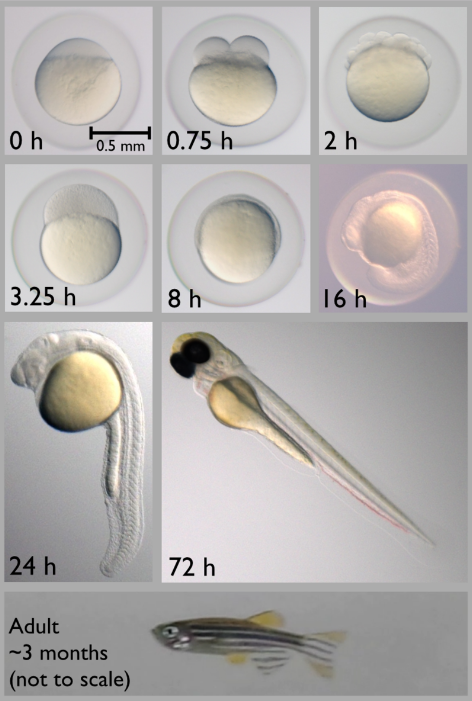
\includegraphics[width=0.4\textwidth]{zebrafish.png}
  \end{center}
  \caption{Stages of zebrafish development.}
\end{wrapfigure}

To study the effect of different drugs being able to model the blood flow is important. For instance, if the drug actually never reaches the infected cells a potentially effective drug might be considered ineffective on wrong ground. 



\subsection{Generating mesh from original MRI images}

{\color{red} Kent: Kan du si noe om hva slags bilder dette er?}

Starting from \texttt{original\_zebrafish.vti} a finite element method mesh can be created using a software called \emph{The Vascular Modeling Toolkit(VMTK)}. VMTK is a collection of libraries and tools for 3D reconstruction, geometric analysis, mesh generation and surface data analysis for image-based modeling of blood vessels.

Installatiion: http://www.vmtk.org/download/ (Use development version!) 

Tutorials: http://www.vmtk.org/tutorials/

1) Select a volume of interest(VOI)
\begin{framed}       
    \texttt{vmtkimagevoiselector -ifile original.vti -ofile voi.vti}
\end{framed}
2) Segmentation
\begin{framed}       
    \texttt{vmtklevelsetsegmentation -ifile voi.vti -ofile levelsets.vti}
\end{framed}
3) Create surface file
\begin{framed}       
    \texttt{vmtkmarchingcubes -ifile levelsets.vti -ofile surf.vtp}
\end{framed}
4) Smoothing of surface
\begin{framed}       
    \texttt{dvmtksurfacesmoothing -ifile surf.vtp -passband 0.1 -iterations 30 -ofile sm\_surf.vtp}
\end{framed}
5) Clip surface
\begin{framed}       
    \texttt{vmtksurfaceclipper -ifile sm\_surf.vtp -ofile cl\_surface.vtp}
\end{framed}
6) Generate mesh
\begin{framed}       
    \texttt{vmtkmeshgenerator -ifile cl\_surface.vtp -ofile zebramesh.vtu -edgelength
1.0}
\end{framed}
7) Convert to dolfin-format
\begin{framed}       
    \texttt{vmtkmeshwriter -ifile zebramesh.vtu -entityidsarray CellEntityIds -ofile zebra\_mesh.xml}
\end{framed}


 \begin{figure}[h!] 
\begin{center}
  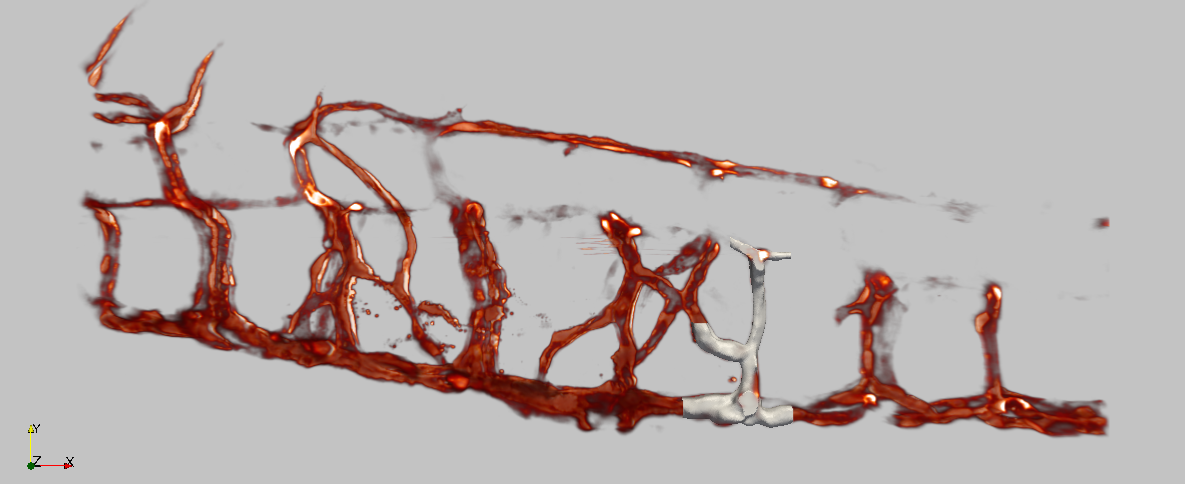
\includegraphics[scale=0.3]{overview2.png}
  \end{center}
  \caption{The circulatory system of a zebrafish where a small part is meshed.}
\end{figure}

\begin{figure}[h!] 
\begin{center}
  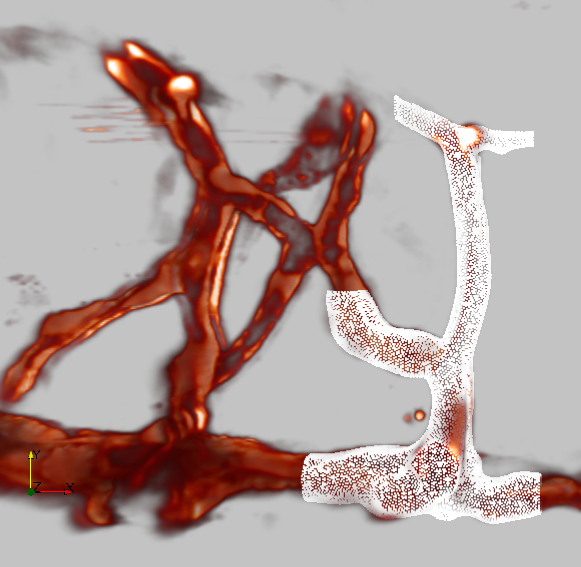
\includegraphics[scale=0.3]{zoomed2.png}
  \end{center}
  \caption{Zooming in to see the meshed region.}
\end{figure}

\subsection{Mathematical formulation}

The blood velocities in a zebrafish are low thus using \emph{Stokes flow} as a model is a fair approximation.

For for geometries with lots of cells using $P_1-P_1$ formulations saves a lot of time and memory, and to even be able to run simulations on your own computer with the \texttt{zebrafish.xml} mesh such a formulation is needed. 


 
Find $u,p \in W,\: W = V \times Q $ such that
\begin{align*}
a((u,p),(v,q)) = L((v,q)) \quad \forall \quad v,q \in W 
\end{align*}
where
\begin{align*}
a((u,p),(v,q)) &= \int_\Omega \nabla u : \nabla v - (\nabla \cdot v)p + (\nabla \cdot u)q + \epsilon \nabla q \cdot \nabla p \: dx \\
L((v,q)) &= \int_\Omega  (v + \epsilon \nabla q) \cdot f \: dx
\end{align*}
Here \(\epsilon = \beta h^2\) and \(\beta\) is some number and \(h\) is the mesh cell size.

Boundary conditions
\begin{align*}
u = 0 \quad &on \quad \partial \Omega_{\text{ no-slip}} \\
\sigma \cdot \mathbf{n} = p_i\mathbf{n} \quad &on \quad \partial \Omega_\text{ opening(i)},\quad i=1,..,5
\end{align*}

\section{Squeezing a postdoc's brain}

We would very much like to squeeze postdoc Erika Lindström's brain. Since she has refused to let us do this with our hands in her office, we must do this on a computer using her brain as our computational domain. The brain will be deformed as a result of the squeezing and to capture this effect we will use a \emph{linear elastic} model. 

A mesh of Erika's brain can be found in the git repository:
 https://github.com/krikarls/fun-with-fem. 
 
 \begin{figure}[h!] 
\begin{center}
  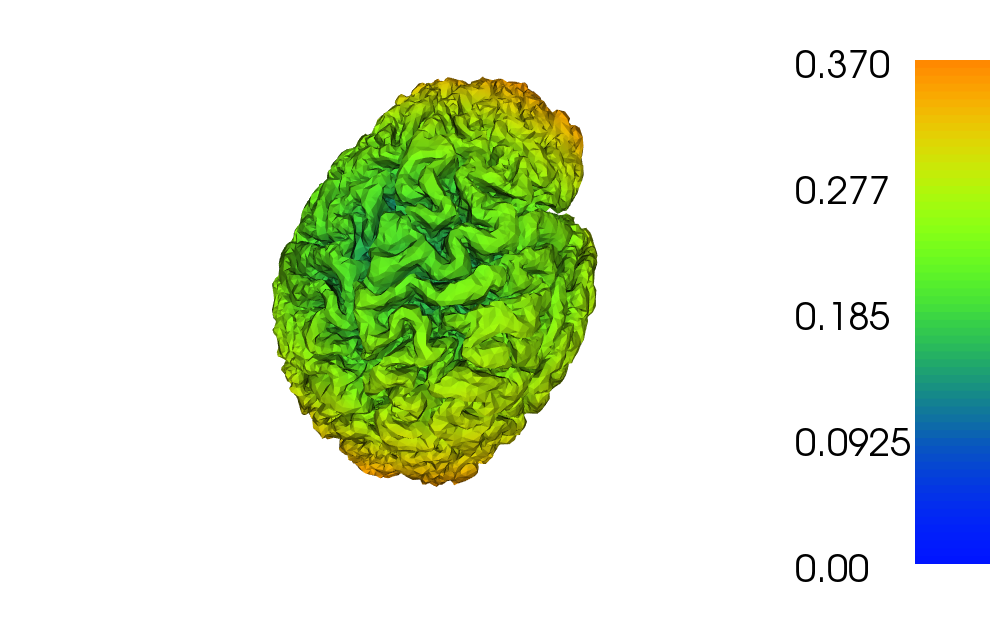
\includegraphics[scale=0.4]{brain.png}
  \end{center}
  \caption{Numerical solution using FEniCS. Displacement measured in $mm$.}
\end{figure}

The brain is not clamped in the skull, but in a sense floating around. This means that we must employ \emph{neumann boundary conditions} on the entire boundary. As we know, there are no unique solution to such a problem since all \emph{rigid motions} satify the equation. So in order to obtain a unique solution we must remove all rigid motions. All the possible rigid motions in 3D are: translations in $x,y,z$-direction and rotations around the corresponding axes. Thus six in total.

An example using \emph{FEniCS} on how to remove these can be found in the same repository as the brain mesh. 

\subsection{Mathematical formulation}

Find $u$ such that 
\begin{align*}
  \int_\Omega  2\mu (\epsilon(u) : \epsilon(v))  +\lambda (\nabla \cdot u) (\nabla \cdot v) \: dx = \int_\Omega f \cdot v \: dx \quad \forall v \in V
\end{align*} 

Boundary conditions
\begin{align*}
\sigma \cdot \mathbf{n} = p\mathbf{n} \quad &on \quad \partial \Omega
\end{align*}

The material parameters for Erika's brain are $E = 16000 $ Pa and $\nu = 0.25$. The Lamè coefficients can be computed according to 
\begin{align*}
\lambda = \frac{E \nu}{(1-2\nu)(1+\nu)} \quad and \quad \mu = \frac{E}{2(1+\nu)}.
\end{align*}
\end{document}
